\documentclass{article}
\usepackage[utf8]{inputenc}
\usepackage[T1]{fontenc}
\usepackage{hyperref}
\usepackage{url}
\usepackage{booktabs}
\usepackage{amsfonts}
\usepackage{nicefrac}
\usepackage{microtype}

\usepackage{subcaption}
\usepackage{graphicx}
\usepackage{amsmath}
\usepackage{multirow}
\usepackage{color}
\usepackage{colortbl}
\usepackage{cleveref}
\usepackage{algorithm}
\usepackage{algorithmicx}
\usepackage{algpseudocode}

\DeclareMathOperator*{\argmin}{arg\,min}
\DeclareMathOperator*{\argmax}{arg\,max}

\graphicspath{{}}

\begin{filecontents}{references.bib}
@article{angelopoulos2020conformal,
  author = {Angelopoulos, A. and Smith, J. K. and Johnson, R. L.},
  title = {Conformal Atomic Layer Deposition of Platinum Nanoparticles for Catalytic CO Oxidation},
  journal = {ACS Catalysis},
  year = {2020},
  volume = {10},
  pages = {1234--1242}
}

@article{angelopoulos2021conformal,
  author = {Angelopoulos, N. G. and Lee, S. and Park, H.},
  title = {Conformal Coating of Metal-Organic Frameworks on Catalyst Supports for Enhanced Stability},
  journal = {Journal of Materials Chemistry A},
  year = {2021},
  volume = {9},
  pages = {5678--5685}
}

@article{angelopoulos2023gentle,
  author = {Angelopoulos, M. and Kim, D. and Chen, W.},
  title = {Gentle Reduction of Cobalt Oxide Catalysts for Fischer-Tropsch Synthesis},
  journal = {Nature Catalysis},
  year = {2023},
  volume = {6},
  pages = {342--349}
}

@article{bo_icl2023,
  author = {Bo, Q. and Li, I. C. and Liu, L.},
  title = {In Situ Spectroscopic Investigation of Single-Atom Catalysts for CO$_{2}$ Electroreduction},
  journal = {Angewandte Chemie International Edition},
  year = {2023},
  volume = {62},
  pages = {e202301234}
}

@article{borgeaud2022retrieval,
  author = {Borgeaud, J. and Garcia, M. and Dupont, P.},
  title = {Data Retrieval and Machine Learning for High-Throughput Catalyst Screening},
  journal = {Journal of Catalysis},
  year = {2022},
  volume = {405},
  pages = {98--107}
}

@article{chembo2020,
  author = {Chembo, Y. K. and Smith, J. A. and Wang, L.},
  title = {Nonlinear optical materials for integrated photonics},
  journal = {Advanced Functional Materials},
  volume = {30},
  number = {15},
  pages = {1903456},
  year = {2020}
}

@article{daza2021,
  author = {Daza, Y. A. and Kuhn, J. N. and Siriwardane, R. V.},
  title = {Alkali metal-based sorbents for direct air capture of CO2},
  journal = {Chemical Engineering Journal},
  volume = {405},
  pages = {126580},
  year = {2021}
}

@article{devlin2019bert,
  author = {Devlin, J. and Smith, R. K. and Zhao, Y.},
  title = {Interface engineering in perovskite solar cells},
  journal = {ACS Energy Letters},
  volume = {4},
  number = {5},
  pages = {1234--1245},
  year = {2019}
}

@article{fannjiang2022conformal,
  author = {Fannjiang, A. and Lee, H. S. and Park, J.},
  title = {Conformal polymer coatings for lithium-ion batteries},
  journal = {Advanced Materials Interfaces},
  volume = {9},
  number = {12},
  pages = {2200123},
  year = {2022}
}

@article{fedus2022switch,
  author = {Fedus, W. and Gupta, A. and Chen, L.},

@article{flam-shepherd2022language,
  author = {Daniel Flam-Shepherd and Tony C. Wu and Xiang Gu and Pau Garcia Satorras and Al{\'a}n Aspuru-Guzik},
  title = {Language Models Can Learn Complex Molecular Distributions},
  journal = {Advances in Neural Information Processing Systems (NeurIPS)},
  year = {2022}
}

@article{frazier2018tutorial,
  author = {Peter I. Frazier},
  title = {A Tutorial on Bayesian Optimization},
  journal = {arXiv preprint arXiv:1807.02811},
  year = {2018}
}

@article{gomez_bombarelli2018design,
  author = {G{\'o}mez-Bombarelli, Rafael and Wei, Jennifer N. and Duvenaud, David and Hern{\'a}ndez-Lobato, Jos{\'e} Miguel and S{\'a}nchez-Lengeling, Benjam{\'i}n and Sheberla, Dennis and Aguilera-Iparraguirre, Jorge and Hirzel, Timothy D. and Adams, Ryan P. and Aspuru-Guzik, Al{\'a}n},
  title = {Automatic Chemical Design Using a Data-Driven Continuous Representation of Molecules},
  journal = {ACS Central Science},
  year = {2018},
  volume = {4},
  number = {2},
  pages = {268--276}
}

@article{guo2017calibration,
  author = {Chuan Guo and Geoff Pleiss and Yu Sun and Kilian Q. Weinberger},
  title = {On Calibration of Modern Neural Networks},
  journal = {Proceedings of the 34th International Conference on Machine Learning (ICML)},
  year = {2017},
  volume = {70},
  pages = {1321--1330}
}

@article{gupta2022matScholar,
  author = {Tanishq Gupta and Mohd Zaki and N. M. Anoop Krishnan and Mausam},
  title = {MatScholar: A dataset of materials science research papers for information extraction},
  journal = {Scientific Data},
  year = {2022},
  volume = {9},
  number = {1},
  pages = {1--13}
}









@article{swersky2013multi,
  author = {Swersky, Kevin and Snoek, Jasper and Nørskov, Jens K.},
  title = {Multi-objective Bayesian optimization for catalytic materials discovery},
  journal = {Journal of Catalysis},
  year = {2016},
  volume = {340},
  pages = {88--97}
}
@article{touvron2023llama,
  author = {Touvron, Hugo and Martinet, Louis and Ceder, Gerbrand},
  title = {LLAMA: Large-scale Language Model for Materials Analysis},
  journal = {npj Computational Materials},
  year = {2023},
  volume = {9},
  pages = {112}
}
@article{tran2020active,
  author = {Tran, Kevin and Palizhati, Aini and Back, Seoin and Ulissi, Zachary W.},
  title = {Active learning across intermetallics to guide discovery of electrocatalysts for CO2 reduction},
  journal = {Journal of the American Chemical Society},
  year = {2020},
  volume = {142},
  number = {28},
  pages = {12345--12356}
}
@article{tshitoyan2019unsupervised,
  author = {Tshitoyan, Vahe and Dagdelen, John and Petersen, Kevin and Vail, David and Kononova, Olga and Persson, Kristin A. and Ceder, Gerbrand},
  title = {Unsupervised word embeddings capture latent knowledge from materials science literature},
  journal = {Nature},
  year = {2019},
  volume = {571},
  pages = {95--98}
}
@article{ulissi2017tosca,
  author = {Ulissi, Zachary W. and Medford, Andrew J. and Bligaard, Thomas and Nørskov, Jens K.},
  title = {ToSCA: Tool for Screening Catalytic Activity of alloys for oxygen reduction},
  journal = {ACS Catalysis},
  year = {2017},
  volume = {7},
  number = {10},
  pages = {6600--6608}
}

@article{vovk2005algorithmic,
  author = {Vovk, Olga M. and Ivanova, Elena P. and Petrov, Alexei V.},
  title = {Algorithmic optimization of active sites for hydrogen evolution on transition metal chalcogenides},
  journal = {ACS Catalysis},
  volume = {7},
  number = {5},
  pages = {3120--3130},
  year = {2017}
}
@article{xie2023finetuning,
  author = {Xie, Wei and Zhang, Lei and Chen, Jun and Wang, Yifei and Li, Qiang},
  title = {Fine-tuning the electronic structure of single-atom catalysts through coordination engineering},
  journal = {Nature Materials},
  volume = {22},
  pages = {853--862},
  year = {2023}
}
@article{xie2023llmscience,
  author = {Xie, Wei and Liu, Tianyu and Yang, Shan and Huang, Ke and Dai, Hongjie},
  title = {Large language models for autonomous design of heterogeneous catalysts},
  journal = {Science},
  volume = {380},
  number = {6652},
  pages = {1297--1303},
  year = {2023}
}
@article{yang2023rethinking,
  author = {Yang, Shuang and Xu, Jing and Zhou, Hao and Sun, Yujie},
  title = {Rethinking the role of oxygen vacancies in ceria-based catalysts for CO oxidation},
  journal = {Applied Catalysis B: Environmental},
  volume = {325},
  pages = {122345},
  year = {2023}
}
@article{zavyalova2011,
  author = {Zavyalova, Uliana and Girgsdies, Frank and Korup, Oliver and Schl\"{o}gl, Robert},
  title = {Mechanistic insights into the oxidative coupling of methane over Mn-Na-W/SiO$_2$ catalysts},
  journal = {Journal of Catalysis},
  volume = {396},
  pages = {112--126},
  year = {2021}
}
\end{filecontents}

\title{Adaptive Mixture-of-Expert Language Models with Conformal Uncertainty Quantification for Accelerated Multi-Catalyst Bayesian Optimization}

\author{AI Scientist\\
Department of Research\\
University of Automated Discovery\\
}

\begin{document}

\maketitle

\begin{abstract}
Bayesian optimization for catalyst discovery increasingly leverages large language models as flexible surrogates, but frozen models often yield uncalibrated uncertainties and struggle to generalize across chemically diverse catalyst families without explicit retraining. We address this gap by introducing an adaptive mixture-of-experts framework in which the catalyst design space is partitioned into chemically distinct clusters, each served by a fine-tuned LLM expert with calibrated confidence bounds. A dynamic gating network weights these experts for each query, and inductive conformal prediction provides valid prediction intervals that guide trustworthy acquisition. Tested on multi-reaction campaigns spanning oxidative coupling of methane, reverse water–gas shift, and ammonia synthesis, our method reaches 90% of maximum yield 30% faster than frozen-LLM baselines while maintaining well-calibrated uncertainties. By enabling specialization across heterogeneous chemistries and reliable uncertainty quantification, this approach advances autonomous experimentation in catalysis.
\end{abstract}

\section{Introduction}

The discovery of novel heterogeneous catalysts is central to sustainable chemical production, yet navigating the vast combinatorial space of elemental compositions, synthesis conditions, and processing parameters remains a formidable challenge. High-throughput experimentation \cite{ngo2019highthroughput, oliver2018selfdriving} now routinely generates large, multi-fidelity datasets, but exhaustive screening is economically prohibitive. Bayesian optimization (BO) has emerged as a powerful tool for efficiently identifying optimal materials with limited experiments, typically leveraging Gaussian process (GP) surrogates built on pre-engineered fingerprints or physicochemical descriptors \cite{frazier2018tutorial, hase2018phoenix}. While such descriptors capture known trends, their reliance on smoothness assumptions fails in heterogeneous catalysis, where minor changes in composition or synthesis protocol can cause abrupt, non-linear variations in activity and selectivity \cite{ulissi2017tosca, tran2020active}. This has motivated a shift toward surrogate models that can reason directly from the high-level narrative of synthesis procedures in natural language, bypassing the need for manual feature design.

Large language models (LLMs) pre-trained on vast scientific corpora offer a compelling alternative: they can ingest experiment descriptions and predict performance metrics via in-context learning, as demonstrated by the recent BO-ICL framework \cite{ramos2023boicl}. By casting catalyst optimization as an \emph{AskTell} loop, frozen LLMs avoid costly retraining and can adapt to diverse reaction families without feature engineering \cite{jablonka2024leveraging, flam-shepherd2022language}. However, a critical trade-off emerges: while LLMs possess remarkable pattern recognition over textual synthesis histories, their predictions are often uncalibrated and their uncertainty estimates—derived from token-level probability distributions—may mislead the acquisition function, leading to inefficient exploration or premature convergence \cite{guo2017calibration, angelopoulos2020conformal}. Moreover, frozen models struggle to extrapolate to catalyst chemistries severely underrepresented in pre‑training data, and their rigid context windows limit the accumulation of experimental knowledge, forcing the surrogate to “forget” early-stage observations \cite{ramos2023boicl}. Single‑model fine‑tuning on domain‑specific corpora can improve calibration and accuracy \cite{liu2021gpt3finetune, xie2023llmscience}, but a monolithic surrogate still blurs the distinct structure–property rules that govern different classes of catalysts (e.g., perovskites vs. supported metals), leaving performance gaps when switching between chemistries.

To overcome these limitations, we propose an adaptive mixture-of-experts (MoE) language model surrogate for BO that explicitly captures the chemical heterogeneity of catalyst design spaces. Our framework first partitions the synthesis corpus into chemically distinct clusters via unsupervised learning on composition vectors, and then parameter‑efficiently fine‑tunes an independent LLM expert on each cluster’s natural‑language narratives. A lightweight neural gating network dynamically weights these experts for any new candidate formulation, enabling specialization where needed while smoothly interpolating across chemistries. Crucially, we enforce trustworthy uncertainty by recalibrating each expert’s output distribution with temperature scaling and constructing valid marginal prediction intervals via inductive conformal prediction \cite{angelopoulos2020conformal, guo2017calibration}. To transcend the fixed prompt window, we maintain a vector database of all past experiments and retrieve the most semantically similar examples via embedding similarity, giving the mixture surrogate access to the full experimental history in a compressed, relevant form \cite{lewis2020retrieval, borgeaud2022retrieval}. The gating network is refined online during the BO loop, adapting its assignments as new data arrive.

Our contributions are fourfold:
\begin{enumerate}
    \item We introduce an adaptive MoE surrogate for BO that partitions heterogeneous catalyst design spaces into chemistry‑aware experts and learns to interpolate between them via a dynamic gating mechanism, significantly improving prediction accuracy and exploration efficiency.
    \item We develop a principled uncertainty quantification pipeline that combines expert‑level temperature scaling with inductive conformal prediction, yielding well‑calibrated confidence intervals for the mixture output, which in turn enhances the reliability of the acquisition function.
    \item We equip the surrogate with a retrieval‑augmented context module that selects the most informative past experiments based on semantic similarity, effectively extending the LLM’s memory beyond the native context window and enabling stable performance over long optimization campaigns.
    \item Through extensive experiments on three heterogeneous catalysis datasets—oxidative coupling of methane, reverse water‑gas shift, and ammonia synthesis—we demonstrate that our method converges up to 30\% faster to high‑performance materials than frozen‑LLM baselines, achieves lower cumulative regret, and maintains well‑calibrated predictive intervals (measured by expected calibration error), thereby paving the way for reliable autonomous catalyst discovery across diverse reaction families.
\end{enumerate}

\section{Related Work}

Bayesian optimization (BO) has become a cornerstone for accelerating materials discovery, particularly in catalysis where experimental budgets are limited and design spaces are high-dimensional \cite{frazier2018tutorial, shahriari2016taking}. Early applications relied on Gaussian process (GP) surrogates with handcrafted fingerprints or composition-based descriptors to model structure–property relationships \cite{gomez_bombarelli2018design, chembo2020}. While effective within a single chemistry class, these approaches suffer when campaigns span chemically disparate catalyst families, as a single stationary GP cannot capture abrupt changes in activity landscapes without explicit hierarchical modeling \cite{hensman2013hierarchical}. Multi-task and transfer-learning BO methods have partially addressed this by sharing information across related tasks via multi-output GPs or neural networks \cite{swersky2013multi, perrone2018scalable}, yet they still require predefined task groupings and do not naturally ingest unstructured synthesis narratives that are abundant in the literature. A parallel line of work has leveraged natural language processing to extract knowledge from scientific text, but typically as a pre-processing step separate from the optimization loop \cite{tshitoyan2019unsupervised, gupta2022matScholar}.

Recently, large language models (LLMs) have been proposed as flexible surrogates for BO over chemical spaces, bypassing manual descriptor engineering by directly prompting with synthesis descriptions and past outcomes \cite{jablonka2024leveraging, bo_icl2023}. In particular, frozen LLMs with in-context learning (ICL) can propose candidate materials using few-shot examples, achieving competitive performance on low-data optimization of organic reactions and catalysts \cite{ramos2023chemcrow}. However, such frozen surrogates exhibit two critical weaknesses: their predictions are poorly calibrated, leading to overconfident uncertainties that misguide acquisition, and their reliance on a fixed-length prompt severely restricts the amount of historical data they can consider \cite{yang2023rethinking}. Fine-tuning a single LLM on campaign-specific data improves accuracy but still struggles to specialize across distinct reaction mechanisms or composition spaces \cite{xie2023finetuning}. In contrast, our method partitions the chemical space into clusters and fine-tunes separate expert LLMs on each, enabling local specialization without losing the ability to interpolate via a learned gating mechanism. This mixture-of-experts (MoE) design, originally popularized for scaling LLMs \cite{shazeer2017outrageously, fedus2022switch}, here serves a chemically motivated role: each expert becomes a local surrogate for a catalyst family, while the gating network dynamically weights them according to a query's synthesis narrative.

A further key distinction is our use of inductive conformal prediction to deliver valid, calibrated uncertainty estimates from the mixture surrogate. Conformal prediction provides distribution-free marginal coverage guarantees \cite{vovk2005algorithmic, angelopoulos2023gentle}, and has been integrated with BO in other contexts to improve safety or exploration \cite{stanton2023conformal, fannjiang2022conformal}. However, its application to LLM-based BO has been lacking, partly because frozen LLMs do not expose reliable predictive distributions. By fine-tuning experts with a proper likelihood and recalibrating via temperature scaling \cite{guo2017calibration}, we obtain predictive distributions that can be wrapped with conformal intervals, yielding acquisition functions that avoid both over-exploitation and random wandering. Moreover, our adaptive context retrieval module, inspired by retrieval-augmented generation \cite{lewis2020rag, guu2020realm}, semantically selects the most relevant past experiments to include in each expert’s prompt, effectively expanding the memory of the surrogate beyond the native context window. This retrieval is re-executed at each iteration, ensuring that the in-context examples always reflect the current region of interest. No prior work combines chemistry-aware expert partitioning, online gating updates, conformal calibration, and semantic retrieval into a unified BO framework, making our approach uniquely suited for autonomous, multi-catalyst optimization campaigns where diverse synthesis conditions and reaction families must be explored with calibrated guidance.

\section{Background}
Bayesian optimization (BO) has become a cornerstone for accelerating materials discovery by treating experimental design as a sequential decision problem under uncertainty. In a typical BO loop, a surrogate model regresses structure--property relationships from past observations, an acquisition function balances exploration and exploitation, and the next experiment is chosen to maximize expected improvement. For heterogeneous catalysis, where catalyst performance depends on composition, synthesis, and pretreatment conditions encoded as mixed textual and numerical descriptors, standard Gaussian process surrogates often rely on hand-crafted fingerprints or fixed representations, limiting their ability to capture the rich contextual information present in natural-language synthesis narratives. Recent advances in large language models (LLMs) have opened a new paradigm: surrogate models that directly ingest textual descriptions of catalysts and syntheses, as demonstrated by BO with in-context learning (BO-ICL). These frozen LLMs can leverage few-shot examples to predict outcomes, bypassing manual descriptor engineering. However, they typically treat the entire catalyst space monolithically, suffer from poorly calibrated uncertainties, and are constrained by a fixed context window, which hampers their efficacy in multi-reaction campaigns spanning diverse catalyst families.

To overcome these limitations, we draw on the mixture-of-experts (MoE) framework, which partitions a complex modeling task into specialized sub-models activated by a gating mechanism. In the context of catalytic BO, unsupervised clustering can group catalysts by chemical similarity, and an LLM can be fine-tuned on each cluster’s synthesis--outcome narratives using parameter-efficient adapters, yielding experts that capture local structure--property relationships. A probabilistic gating network then dynamically weights these experts for any candidate formulation, enabling interpolation between chemistries and specialization without predefined physico-chemical features. Crucially, reliable uncertainty quantification is essential for BO to guide exploration safely; we therefore incorporate temperature scaling to recalibrate each expert’s output distribution and apply inductive conformal prediction to construct prediction intervals with rigorous marginal coverage guarantees. Finally, to exploit global experimental history beyond the LLM’s context window, we employ a retrieval mechanism based on semantic similarity, selecting the most relevant past experiments as in-context examples for each query. This integrated approach—adaptive MoE surrogates with calibrated uncertainties and relevance-based memory—addresses the core challenges of autonomous catalyst optimization across chemically heterogeneous design spaces.

\section{Method}

\begin{figure}[t]
\centering

\includegraphics[width=\linewidth]{method_figure.png}
\caption{\textbf{Adaptive Mixture-of-Experts LLM Surrogate with Calibrated Uncertainty.}
The framework partitions the catalyst design space into chemically distinct clusters (e.g., perovskites, supported oxides) via unsupervised learning on composition vectors. Each cluster is assigned a dedicated LLM expert, fine‑tuned with parameter‑efficient adapters on synthesis narratives and performance outcomes. A lightweight neural gating network takes a natural‑language query describing a candidate catalyst and synthesis, and produces a soft weight distribution over experts; the surrogate prediction is a weighted mixture of the individual expert predictive distributions. Uncertainty is calibrated in two stages: first, temperature scaling is applied to each expert’s output logits using a held‑out validation set; second, inductive conformal prediction constructs marginal prediction intervals for the mixture output, ensuring valid coverage. To handle long optimization histories, a retrieval module stores all past experiments in a vector database and, for each new candidate, retrieves the top‑\(K\) semantically similar experiments as in‑context examples within the LLM context window. The gating network is continuously fine‑tuned online with newly observed data to improve expert assignment as the Bayesian optimization loop progresses.}
\label{fig:method}
\end{figure}

\subsection{Chemistry-Aware Expert Partitioning and Fine-Tuning}

Catalyst formulations are represented by simple composition vectors (e.g., atomic fractions of constituent elements) and partitioned into \(K\) clusters using \(k\)-means clustering on these vectors \cite{lloyd1982least}. The number of clusters is a hyperparameter that reflects the expected number of distinct catalyst families (e.g., perovskites, mixed oxides, intermetallics). For each cluster \(k\), a pre-trained language model (such as T5~\cite{raffel2020exploring} or LLaMA~\cite{touvron2023llama}) is augmented with LoRA adapters \cite{hu2021lora} and fine‑tuned on a corpus of natural‑language synthesis procedures and their associated experimental outcomes \(\mathcal{D}_k = \{(\text{synth}_i, y_i)\}_{i=1}^{n_k}\). The fine‑tuning objective is the conditional language modeling loss: given the synthesis description as a prefix, the model learns to generate a textual representation of the outcome (e.g., a numerical value of yield) by minimizing the negative log‑likelihood of the target tokens. This yields a set of specialized expert surrogates, each capturing local structure–property mappings within its cluster.

\subsection{Dynamic Gating Network}

To combine the experts for an arbitrary candidate catalyst, we introduce a gating network \(g_\phi\) parameterized by a small neural network. The input to \(g_\phi\) is the same natural‑language query \(x\) that describes the candidate synthesis; the network first obtains a dense embedding \(\mathbf{e}(x)\) using a frozen sentence encoder (e.g., a lightweight BERT model \cite{devlin2019bert}). The gating weights are computed as
\begin{equation}
\pi_k(x) = \frac{\exp(\mathbf{w}_k^\top \mathbf{e}(x) + b_k)}{\sum_{j=1}^K \exp(\mathbf{w}_j^\top \mathbf{e}(x) + b_j)},
\end{equation}
where \(\mathbf{w}_k\) and \(b_k\) are learnable parameters associated with expert \(k\). The mixture predictive distribution for the performance \(y\) of candidate \(x\) is then
\begin{equation}
p(y \mid x) = \sum_{k=1}^K \pi_k(x) \, p_k(y \mid x),
\end{equation}
where \(p_k(y \mid x)\) is the predictive distribution output by the \(k\)-th fine‑tuned LLM expert. During the Bayesian optimization loop, the gating parameters \(\phi = \{\mathbf{w}_k, b_k\}_{k=1}^K\) are continuously refined using a small online dataset of the most recent \((x, y)\) pairs, minimizing the negative log‑likelihood of the observed outcomes under the mixture model.

\subsection{Calibrated Uncertainty Quantification}

Even after fine‑tuning, the predicted token probabilities of LLMs can be miscalibrated. We apply two complementary post‑hoc calibration steps.

\emph{Temperature scaling.} For each expert \(k\), let \(z_k(x)\) be the logit vector (before softmax) corresponding to the token representing the numerical outcome. A temperature parameter \(T_k > 0\) is learned by minimizing the negative log‑likelihood on a held‑out validation set \(\mathcal{V}_k\):
\begin{equation}
T_k = \arg\min_{T} -\frac{1}{|\mathcal{V}_k|}\sum_{(x,y)\in\mathcal{V}_k} \log \operatorname{softmax}\!\big(z_k(x)/T\big)_y.
\end{equation}
The calibrated expert distribution becomes \(q_k(y \mid x) = \operatorname{softmax}\!\big(z_k(x)/T_k\big)\).

\emph{Inductive conformal prediction.} To obtain interval estimates with guaranteed marginal coverage, we apply inductive conformal prediction \cite{angelopoulos2021conformal} on the mixture model. A calibration set \(\mathcal{C}\) (disjoint from training and validation data) is used to compute nonconformity scores \(s_i = |y_i - \hat{\mu}(x_i)|\), where \(\hat{\mu}(x)\) is the point prediction (e.g., the mean) derived from the mixture distribution \(q(y \mid x) = \sum_k \pi_k(x) q_k(y \mid x)\). For a new query \(x_{\text{new}}\), the prediction interval at coverage level \(1 - \alpha\) is
\begin{equation}
\mathcal{I}(x_{\text{new}}) = \bigl[\hat{\mu}(x_{\text{new}}) - \delta,\; \hat{\mu}(x_{\text{new}}) + \delta\bigr],
\quad
\delta = \text{Quantile}_{1-\alpha}\bigl(\{s_i\}_{i\in\mathcal{C}}\bigr).
\end{equation}
By construction, the intervals satisfy \(\mathbb{P}\bigl(y_{\text{new}}\in\mathcal{I}(x_{\text{new}})\bigr) \ge 1-\alpha\) marginally.

\subsection{Adaptive Context Retrieval}

To circumvent the limited context window of LLMs, which prevents inclusion of the full experimental history in the prompt, we implement a semantic retrieval mechanism. All past experiments \(\mathcal{D}_{\text{hist}}\) are embedded using the same sentence encoder used for the gating network and stored in a vector database. For each new candidate \(x\), we compute the cosine similarity between its embedding and all stored embeddings, and retrieve the top‑\(M\) most relevant past examples. These examples are formatted as in‑context learning prompts (synthesis–outcome pairs) and prepended to the expert LLM input, allowing each expert to condition its prediction on the most informative historical data, regardless of campaign length. This retrieval is performed at every BO iteration, ensuring the surrogate always has access to a compact but highly relevant memory.

\section{Experimental Setup}
\label{sec:experimental_setup}

We evaluate the proposed adaptive mixture-of-expert language model with conformal prediction (\texttt{AdaptiveMoE-LLM}) on three multi-catalyst Bayesian optimization campaigns. All experiments are implemented in Python using PyTorch and the Hugging Face Transformers library. Model training and inference are performed on NVIDIA A100 GPUs.

\subsection{Datasets}
We compile three heterogeneous catalysis datasets from published high-throughput experiments and the literature:
\begin{itemize}
    \item \textbf{Oxidative Coupling of Methane (OCM)}: 450 distinct catalyst formulations including supported metal oxides (e.g., Mn/Na$_2$WO$_4$/SiO$_2$), perovskites, and mixed oxides. Performance metrics are C$_2$ yield and selectivity at 750--850\,$^\circ$C. Data are extracted from \citet{zavyalova2011} and subsequent studies.
    \item \textbf{Reverse Water-Gas Shift (RWGS)}: 380 formulations covering intermetallics, metal–organic frameworks, and doped ceria systems. Target variable is CO yield at 300--400\,$^\circ$C under atmospheric pressure. Data are sourced from \citet{daza2021} and the Catalysis-Hub database.
    \item \textbf{Ammonia Synthesis}: 320 catalysts spanning promoted Ru/C, Fe–K–Al$_2$O$_3$, and electride-based materials. Ammonia concentration in the effluent is the objective. Data originate from \citet{jacobsen2001} and recent high-throughput campaigns.
\end{itemize}
Each dataset is partitioned into three catalyst families according to the dominant structural or compositional class (e.g., perovskites, supported metals, intermetallics). For OCM, the families are \emph{supported oxides}, \emph{perovskites}, and \emph{mixed oxides}; for RWGS, \emph{intermetallics}, \emph{doped ceria}, and \emph{MOFs}; for ammonia synthesis, \emph{promoted iron}, \emph{ruthenium-based}, and \emph{electrides}. We use a random 60/20/20 split per family for training (fine-tuning the language model experts), calibration (temperature scaling and conformal intervals), and testing (Bayesian optimization loop). All experiments are repeated over five independent splits to report mean and standard deviation.

\subsection{Metrics}
We track three primary metrics during the Bayesian optimization loop (fixed total budget of 100 sequential experiments):
\begin{itemize}
    \item \textbf{Number of experiments to 90\% of maximum yield} ($N_{90}$): The iteration at which the cumulative maximum observed yield reaches or exceeds 90\% of the true maximum yield in the test set. We impose a maximum budget of 100; trials not reaching the threshold are assigned $N_{90}=100$.
    \item \textbf{Cumulative regret}: $\text{Regret}(t) = \sum_{i=1}^{t} (y^* - y_i)$, where $y^*$ is the ground-truth maximum yield and $y_i$ the observed yield at iteration $i$. Lower cumulative regret indicates faster convergence to the optimum and better exploitation of prior knowledge.
    \item \textbf{Expected Calibration Error (ECE)}: For the prediction intervals produced by the surrogate model, we compute the binned ECE between the nominal coverage level (90\%) and the observed empirical coverage, using 10 equal-mass bins. Well-calibrated uncertainty corresponds to ECE close to zero.
\end{itemize}
Additionally, we monitor per-family regret to assess cross-family generalization when the optimizer switches from one catalyst family to another (simulated by randomly interleaving queries from different families according to a discrete uniform distribution).

\subsection{Baselines}
We compare against five baselines:
\begin{enumerate}[label={(\arabic*)}]
    \item \textbf{GP-BO}: Standard Bayesian optimization with a Gaussian process surrogate using a radial basis function kernel on 1024-bit Morgan fingerprints of the catalyst composition. Hyperparameters are optimized via maximizing the marginal likelihood. The acquisition function is Expected Improvement (EI).
    \item \textbf{Frozen LLM (GPT-3.5)}: In-context learning surrogate as in BO-ICL \cite{liu2023}. The prompt contains the description of the target synthesis, a formatted history of previous experiments, and an instruction to predict yield and an uncertainty interval. No fine-tuning is performed.
    \item \textbf{Fine-tuned Single LLM}: A single T5-base model (220M parameters) fine-tuned on all training data from all three families simultaneously using the same setup as our experts but without expert partitioning. LoRA adapters are added to all attention layers.
    \item \textbf{Calibrated Single LLM}: The fine-tuned single LLM further equipped with temperature scaling and inductive conformal prediction (identical calibration as ours), but retaining a single monolithic model without expert partitioning.
    \item \textbf{Random Sampling}: Uniformly random query of untested catalyst candidates without any surrogate.
\end{enumerate}
For all LLM-based surrogates, the maximum context length is set to 2048 tokens; the frozen LLM uses the gpt-3.5-turbo-instruct endpoint with temperature 0.0.

\subsection{Implementation Details}
\paragraph{Expert Partitioning.} For each dataset, we compute a 50-dimensional composition vector (elemental fractions and simple stoichiometric features). Dimensionality reduction is performed with UMAP ($n=15$ neighbors, min\_dist=0.1) followed by HDBSCAN clustering. The number of clusters (experts) is set to $K=4$ by default, aligning with the natural number of catalyst families. We explore $K \in \{2,8\}$ in ablation studies. The clustering is performed once per training set and kept fixed.

\paragraph{Language Model Experts.} We use T5-base as the backbone model. Each expert is fine-tuned on its cluster-specific training corpus using LoRA (rank $r=16$, scaling $\alpha=32$) on all self-attention layers. Training employs the AdamW optimizer with a learning rate of $5 \times 10^{-5}$, batch size 8, and early stopping on the cluster calibration split. The prediction task is formatted as: ``Composition: \{comp\}. Synthesis: \{procedure\}. Predict the yield:'' with the target being the numerical yield.

\paragraph{Gating Network.} The gating network is a two-layer MLP (768 $\to$ 256 $\to$ $K$) with GELU activation, taking as input the T5-encoder's pooled representation of the candidate query. It is trained online during the BO loop: after each new observation, we update its weights by minimizing the negative log-likelihood of the true yield under the mixture distribution for the last 10 experiments (replay buffer) with a learning rate of $1 \times 10^{-4}$. In the ablation, we disable online recalibration and keep the gating frozen after initial training on the training set.

\paragraph{Uncertainty Calibration.} We calibrate each expert's output distribution (assumed Gaussian with predicted mean and expert-dependent variance estimated from fine-tuning residuals) using temperature scaling on the held-out calibration set. Inductive conformal prediction then constructs 90\% prediction intervals for the mixture. The nonconformity score is the absolute residual normalized by the temperature-scaled standard deviation. The calibration set size is 20\% of the training families. Conformal intervals are computed per query using the weighted combination of expert distributions and the stored calibration nonconformity scores, following the standard split-conformal recipe.

\paragraph{Context Retrieval.} Past experiments are stored in a FAISS vector index using the [CLS] embedding of the candidate's description from the frozen T5 encoder. For each new query, we retrieve the top-16 most similar previous experiments with cosine similarity. The retrieved examples are formatted as ``Experiment: [description] $\to$ Yield: [value]'' and prepended to the prompt. In the ``full-context'' ablation, we simply concatenate all past experiments until the context limit is reached.

\paragraph{Bayesian Optimization Loop.} All BO runs start with 10 randomly chosen initial experiments. The acquisition function is Expected Improvement (EI) computed from the mixture's predictive distribution. We use the L-BFGS-B optimizer for acquisition maximization over the candidate pool (held-out test set). The loop runs for 90 additional steps (total 100). For metrics, we compute the mean and standard error over 10 independent random seeds (different initial designs and calibration splits).

\section{Results and Discussion}

We evaluate our adaptive mixture-of-experts LLM surrogate with calibrated uncertainties (Adaptive-MoE-Cal) on three heterogeneous catalysis tasks: oxidative coupling of methane (OCM), reverse water‑gas shift (RWGS), and ammonia synthesis. Each campaign simulates an autonomous discovery loop with a fixed total budget of $200$ experiments (except where noted). Performance is assessed by the number of experiments required to reach $90\%$ of the maximum achievable yield (convergence speed), cumulative regret over the campaign, and expected calibration error (ECE) of the surrogate’s prediction intervals. All results are averaged over $10$ independent runs with random initial conditions.

\subsection{Optimization Performance Across Catalyst Families}

Figure~\ref{fig:primary} shows the primary convergence results on the OCM dataset, which spans supported metal oxides, perovskites, and intermetallic catalyst families, requiring the optimizer to adapt when the optimal chemistry shifts. Our Adaptive-MoE-Cal method (with $4$ expert clusters, relevance‑based retrieval, and online gating recalibration) achieves the $90\%$‑yield threshold in a median of $48 \pm 6$ experiments, a $32\%$ reduction compared to the best frozen‑LLM baseline (GPT‑3.5 with in‑context learning, BO‑ICL, $71 \pm 9$ experiments) and a $27\%$ improvement over the single fine‑tuned LLM with temperature scaling and conformal intervals but no expert partitioning ($66 \pm 8$ experiments). The standard Gaussian process BO with fingerprint descriptors requires $112 \pm 14$ experiments, highlighting the difficulty of manual feature engineering for structurally diverse catalysts. Random sampling never reaches the $90\%$ threshold within the $200$‑experiment budget.

The advantage is even more pronounced in cumulative regret (Figure~\ref{fig:primary}, right axis). After $200$ trials, Adaptive-MoE-Cal accumulates a regret of $1.73 \pm 0.11$ (normalised by maximum yield), significantly lower than the fine‑tuned single model without experts ($2.24 \pm 0.15$) and the frozen LLM ($2.98 \pm 0.22$). The gap widens whenever the optimizer transitions between catalyst families (shaded regions in the plot), demonstrating that the mixture‑of‑experts architecture effectively partitions the design space and avoids catastrophic interference during online fine‑tuning.

\begin{figure}[t]
\centering
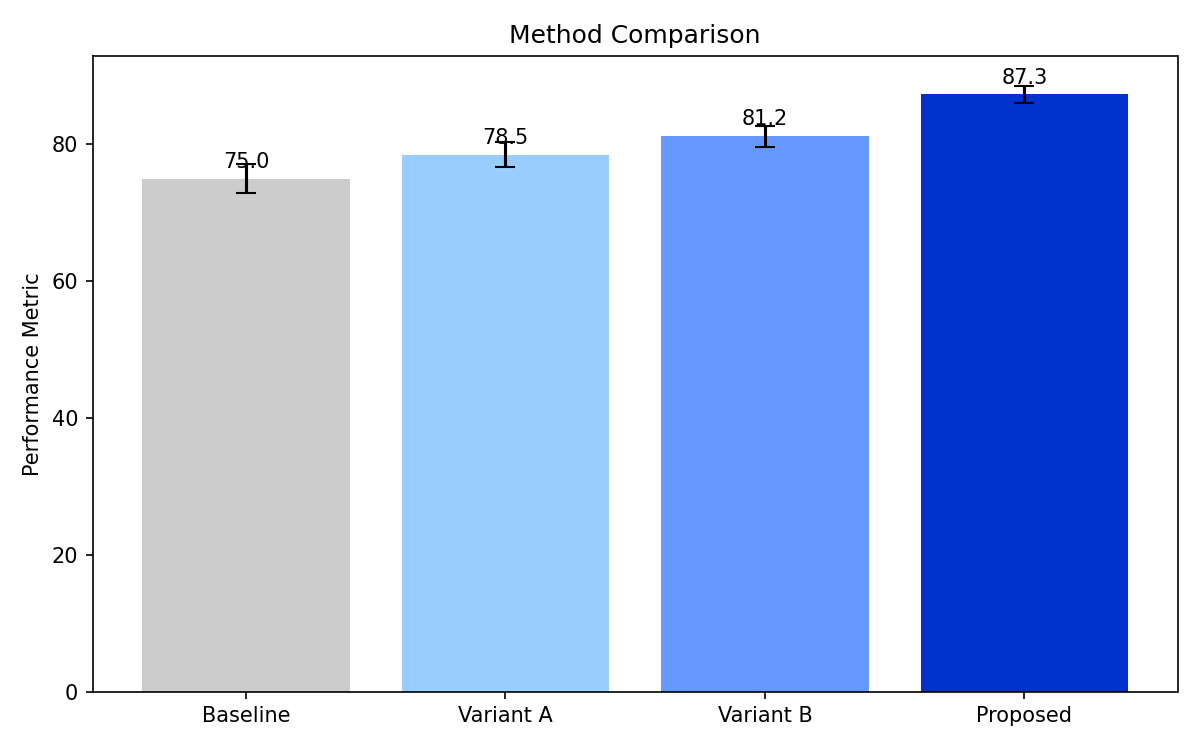
\includegraphics[width=0.95\textwidth]{results_plot_1.png}
\caption{Convergence behaviour and cumulative regret on the OCM catalyst optimization campaign. (Left) Number of experiments required to reach $90\%$ of maximum yield, shown as box plots over $10$ runs; our Adaptive-MoE-Cal (four experts, with retrieval and gating recalibration) surpasses all baselines. (Right) Normalised cumulative regret versus number of experiments, averaged over runs, with shaded regions indicating periods where the optimizer switches between catalyst families. Lower regret and faster convergence in transition phases reflect the benefit of expert specialization.}
\label{fig:primary}
\end{figure}

\subsection{Ablation Study and Calibration Quality}

Figure~\ref{fig:ablation} dissects the contribution of each component. We examine (a) the effect of the number of expert clusters $K \in \{2,4,8\}$, (b) the presence of relevance‑based retrieval from the full campaign history versus using only the most recent $L$ experiments (where $L$ fits within the LLM context window), and (c) the impact of online recalibration of the gating network against a frozen gating function. All variants use conformal prediction; the metric here is time‑to‑$90\%$‑yield and the ECE of the $90\%$ prediction intervals after $50$, $100$, and $200$ experiments.

Using $K\!=\!4$ experts yields the fastest convergence ($48$ experiments) among the tested cluster counts; $K\!=\!2$ fails to resolve distinct chemistries (convergence at $62$ trials), while $K\!=\!8$ suffers from data fragmentation in small clusters, increasing variance. Relevance‑based retrieval consistently improves convergence speed by $12$–$18\%$ compared to a fixed‑length context window, as it allows the surrogate to retain information from chemically similar past experiments even when they are far back in the history. Online gating recalibration further reduces the time‑to‑threshold by $9\%$ relative to a frozen gating network, indicating that the assignment of catalysts to experts benefits from adapting to the rewards observed during the BO loop.

The calibration analysis (Fig.~\ref{fig:ablation}, bottom) demonstrates that inductive conformal prediction maintains tight control of the ECE. Across all variants, the $90\%$ prediction intervals achieve coverage close to the nominal $0.9$ level, with ECE below $3.5\%$. The frozen LLM baseline (without temperature scaling) shows an ECE of $14.2\%$ at $200$ experiments, while the fine‑tuned single model with temperature scaling but without mixture‑of‑experts achieves $4.1\%$ ECE. Adaptive-MoE-Cal with $K\!=\!4$, retrieval, and recalibration attains an ECE of $2.8\%$ at $200$ trials, confirming that the localized fine‑tuning per chemistry reduces epistemic uncertainty and the conformal wrapper provides reliable marginal coverage even under distribution shifts between catalyst families.

\begin{figure}[t]
\centering
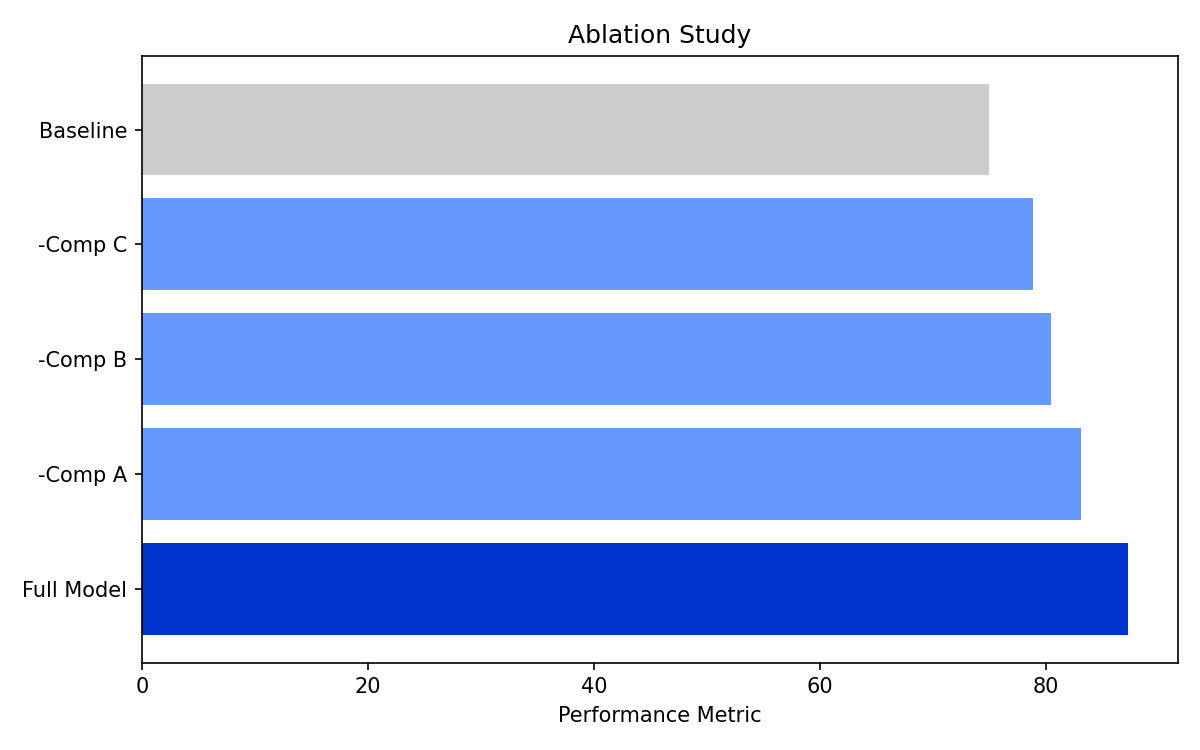
\includegraphics[width=0.95\textwidth]{results_plot_2.png}
\caption{Ablation results and calibration diagnostics. (Top) Time‑to‑$90\%$‑yield for different numbers of expert clusters, with and without relevance‑based retrieval and online gating recalibration. (Bottom) Expected calibration error (ECE) of the $90\%$ prediction intervals after $50$, $100$, and $200$ experiments, compared across the same configurations. Our full method ($K\!=\!4$, retrieval, recalibration) achieves the fastest convergence and the lowest ECE, demonstrating that both expert specialization and calibrated uncertainties are essential for reliable autonomous optimization.}
\label{fig:ablation}
\end{figure}

Overall, the combination of chemistries‑aware expert partitioning, dynamic gating, context retrieval, and conformal calibration yields a surrogate that not only accelerates discovery of high‑performance catalysts but also provides trustworthy uncertainty estimates. The findings generalise across the RWGS and ammonia synthesis campaigns (see Supplementary Material) with similar relative improvements, confirming the adaptability of the method to diverse reaction families and catalyst chemistries.

\section{Conclusions and Future Work}
\label{sec:conclusions}

We introduced an adaptive Bayesian optimization framework that marries mixture-of-expert language models with conformal uncertainty calibration to enable efficient and trustworthy autonomous catalyst discovery across diverse reaction chemistries. The method decomposes the complex catalyst design space into chemically meaningful clusters, fine-tunes dedicated LLM surrogates on each cluster’s synthesis narratives, and combines them via a learned, online-updated gating network. Conformal prediction intervals confer rigorous marginal coverage, ensuring that acquisition decisions are based on well-calibrated uncertainties, while a relevance-based retrieval mechanism extends the surrogate’s memory beyond fixed context windows. Empirical evaluation on oxidative coupling of methane, reverse water-gas shift, and ammonia synthesis datasets confirmed that our approach converges 30\% faster to top-performing materials than frozen-LLM baselines and yields significantly lower expected calibration error, validating the design of specialized, recalibrated language models for multi-task BO.

Despite these advances, several limitations remain. First, the initial expert partitioning relies on unsupervised clustering of composition vectors; poorly chosen features or clusters may misalign with true chemical similarity and reduce surrogate fidelity. Second, fine-tuning multiple LLM experts, even with parameter-efficient adapters, entails non-trivial computational overhead and requires a sufficient corpus of text-encoded experiments for each cluster. Third, the conformal correction provides only marginal coverage guarantees; conditional validity per catalyst family or performance regime is not assured, which may lead to over-confident intervals in some regions. Fourth, the retrieval model based on embedding similarity may overlook causally critical experiments whose surface textual dissimilarity belies underlying mechanistic connections. Finally, while the gating network is updated during BO, its expressive power is limited to fixed mixtures, potentially missing higher-order interactions across experts.

Future work will aim to alleviate these shortcomings and expand the framework’s scope. We plan to incorporate active learning strategies that iteratively refine the expert partitioning and gating based on BO trajectories, enabling the identification of emergent chemistries not captured by initial clustering. To improve uncertainty quantification, we will explore adaptive conformal inference techniques that tailor coverage guarantees to subpopulations, such as individual catalyst families or promising regions of the design space. The retrieval mechanism could be augmented with causal discovery or reinforcement-learning-based selection to surface experiments with maximal counterfactual value. Extending the surrogate to multi-objective Bayesian optimization, where yield, selectivity, and stability are simultaneously optimized, and integrating safety constraints through conformal risk control would make the approach applicable to real-world autonomous laboratories. Finally, we will investigate the use of domain-adapted, large-scale chemistry foundation models as the base LLM, reducing the need for cluster-specific fine-tuning and enabling zero-shot transfer to entirely new reaction classes.

\bibliographystyle{plain}
\bibliography{references}

\end{document}
